\chapter{Results}\label{ch:results}

During the training and testing stages, a number of plots have been made in order to visualize any outliers, along with a list of any anomalies the network has found. Note that all plots in this chapter are based on 1\% of the users.

The \(y\) value resulting from function~\ref{eq:y}, where the IQR is calculated over the training set, can be seen in Figure~\ref{fig:iqr_scale}. As can be seen in the figure, there are quite a few outliers, some of which having errors that fall far beyond the cutoff value of 1.5. From this, it can be concluded that at least some outliers are being found. The \(y\) values also tend to be very low, with around 90\% being 1.0 or lower. This shows that the network is relatively successful at modeling user behavior, as its predictions' errors are very close to the training set's errors. A network that is unsuccessful at this would have a lot of high \(y\) as a result of the bad predictions.

\begin{figure}
	\begin{center}
		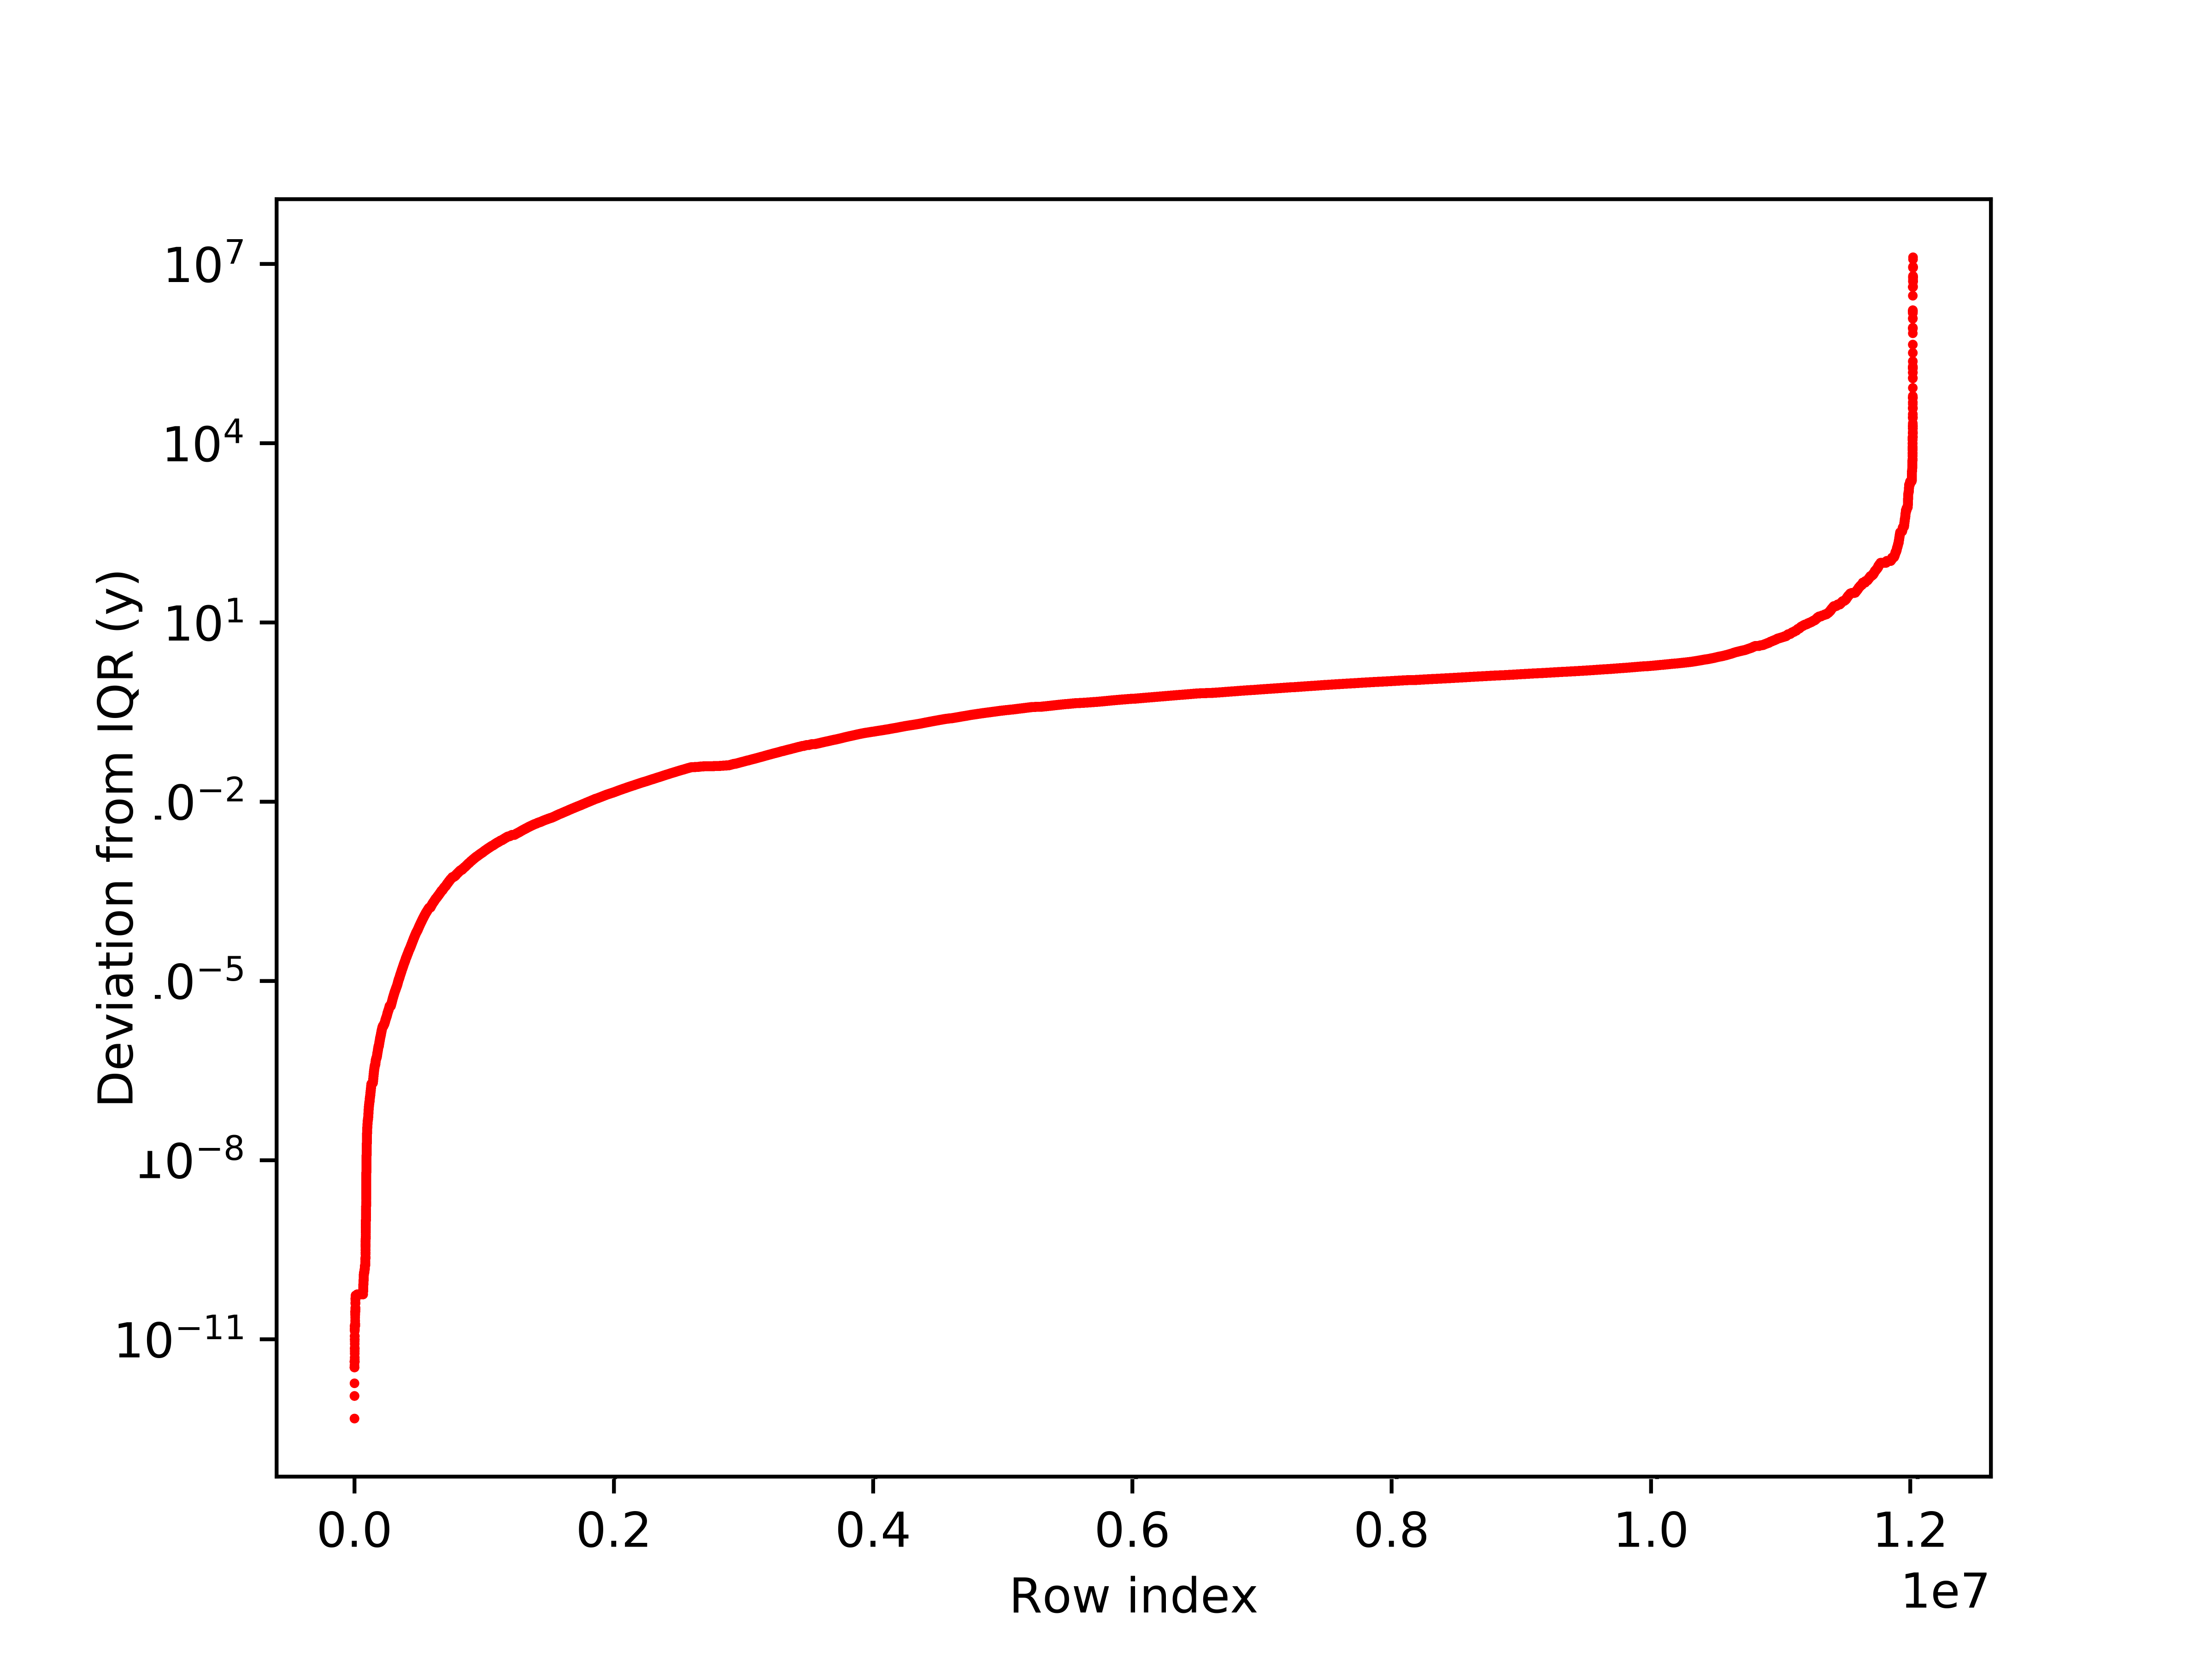
\includegraphics[scale=1.6]{results/all_deviations}
	\end{center}
	\caption{The deviations \(y\) (function~\ref{eq:y}) of the mean squared errors of all predicted test set feature vectors compared to the actual feature vectors. The IQR has been calculated over the training set using the same method of predicted vs actual mean squared error.~\label{fig:iqr_scale}}
\end{figure}

Focussing on the highest offending users allows us to see more clearly why the network thought certain users were deemed anomalies and whether the network may have been right. The highest offending users are the users responsible for the highest offending actions, which are the actions with the highest errors compared to the predictions the network made.

In Figure~\ref{fig:time_since_last_access} a closer look is taken at the time since the last network access for the top 10 highest offending users. This clearly shows some very big deviations from users' times since their last network access. For example, U41 consistently has a very low time since last access, as can be seen from the box plot being very small and concentrated around that area. However, there is a significant deviation from this user's normal behavior, which the network has probably flagged as a deviation. The same goes for other users like U102 and U72, changing their behavior a lot, while \enquote{normal} users like U34, U107 and U119 keep their time since last access consistent. U41's pause only took 2 weeks, which can easily be explained by a vacation, a period of sickness or any other reason for taking a short break. However, this is something that is still worth investigating, as this could also be an abandoned account being picked up by a different (potentially malicious) user.

\begin{figure}
	\begin{center}
		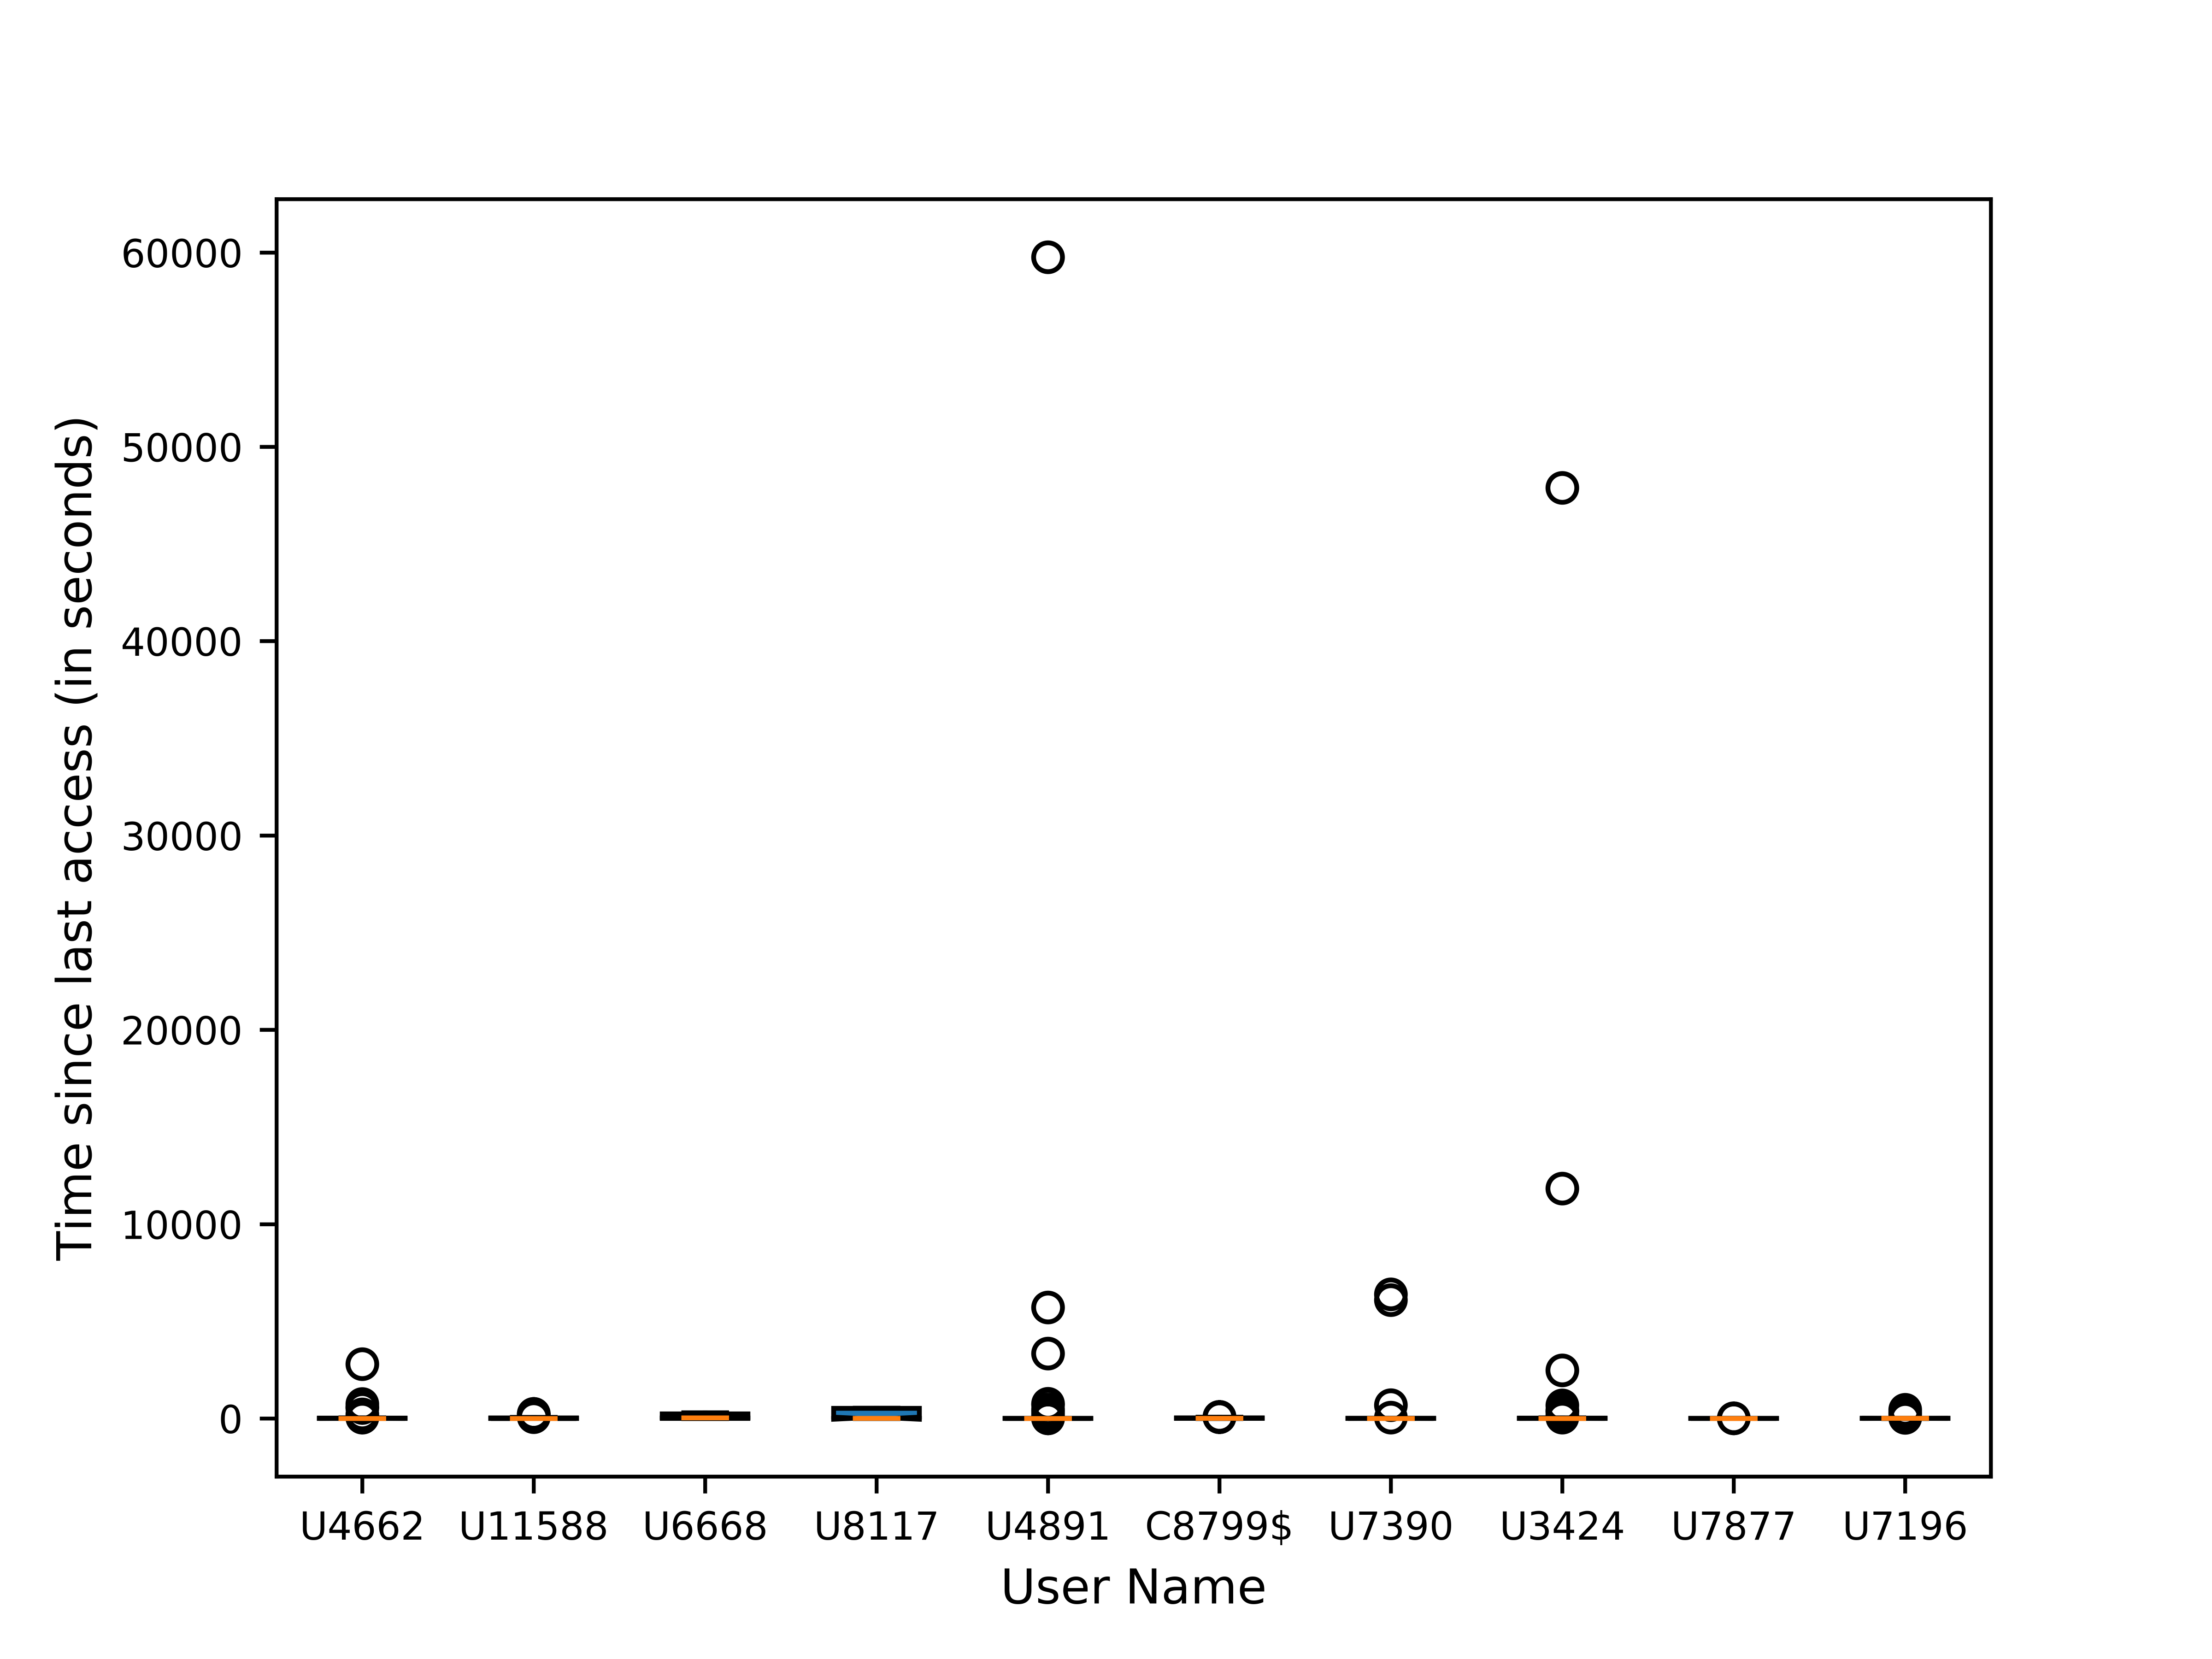
\includegraphics[scale=1.6]{results/highest_offender_time_since_last_access}
	\end{center}
	\caption{The top 10 highest offenders' seconds since last access. Actions with the highest errors aren't necessarily high because of the time since last access metric (U34, U107).~\label{fig:time_since_last_access}}
\end{figure}

The highest offending (highest mean squared error value) feature vector's predicted vs actual action are shown in Table~\ref{tab:predicted_vs_actual_top}. In this table (and following tables) features that are integers and not floats have been depicted as integers, as all but the \(percentage\_failed\_logins\) and \(time\_since\_last\_access\) features are integers. Any predictions made by the network are trimmed to 3 decimal points.

%cSpell:words REMOTEINTERACTIVE
As can be seen, the action in Table~\ref{tab:predicted_vs_actual_top} itself isn't very weird, simply using a different method of authentication, a different method of logging in and a different authentication orientation. These methods themselves are not inherently anomalies, but the network learned that these actions are rarely made by the user, assigning a value of 0.000 to \(auth\_type\_0 \) (NTLM), \(logon\_type\_7 \) (REMOTEINTERACTIVE) and \(auth\_orientation\_2 \) (TGS). The network also assigned values of 0.999 or higher to a single action in all of these enums, pointing to the user almost always logging in using these exact methods. When compared to the user's previous logins in Table~\ref{tab:prev_logins}, the last action really stands out as different.

\begin{table}[htbp]
	\centering
	\caption{The predicted features vs the actual features of the top offending feature set by U399 (precise to 3 decimals)}\label{tab:predicted_vs_actual_top}
	\begin{tabular}{lll}
		Label & Actual & Predicted \\ \midrule
		time\_since\_last\_access & 0.060 & 0.011 \\
		domains\_delta & 0 & 0.000 \\
		dest\_users\_delta & 1 & 0.000 \\
		src\_computers\_delta & 1 & 0.000 \\
		dest\_computers\_delta & 1 & 0.000 \\
		percentage\_failed\_logins & 0.001 & 0.000 \\
		success\_failure & 1 & 0.999 \\
		auth\_type\_0 & 0 & 0.000 \\
		auth\_type\_1 & 0 & 1.000 \\
		auth\_type\_2 & 0 & 0.000 \\
		auth\_type\_3 & 0 & 0.000 \\
		auth\_type\_4 & 0 & 0.000 \\
		auth\_type\_5 & 0 & 0.000 \\
		auth\_type\_6 & 0 & 0.000 \\
		auth\_type\_7 & 0 & 0.000 \\
		auth\_type\_8 & 0 & 0.000 \\
		auth\_type\_9 & 1 & 0.000 \\
		auth\_type\_10 & 0 & 0.000 \\
		logon\_type\_0 & 0 & 0.000 \\
		logon\_type\_1 & 0 & 0.000 \\
		logon\_type\_2 & 0 & 0.000 \\
		logon\_type\_3 & 0 & 0.999 \\
		logon\_type\_4 & 0 & 0.000 \\
		logon\_type\_5 & 0 & 0.000 \\
		logon\_type\_6 & 0 & 0.000 \\
		logon\_type\_7 & 1 & 0.000 \\
		logon\_type\_8 & 0 & 0.000 \\
		auth\_orientation\_0 & 0 & 0.999 \\
		auth\_orientation\_1 & 0 & 0.000 \\
		auth\_orientation\_2 & 1 & 0.000 \\
		auth\_orientation\_3 & 0 & 0.000 \\
		auth\_orientation\_4 & 0 & 0.000 \\
		auth\_orientation\_5 & 0 & 0.000
	\end{tabular}
\end{table}

\begin{table}[htbp]
	\centering
	\caption{The highest offending user's last 30 logins before the anomaly and the anomaly last}\label{tab:prev_logins}
	\resizebox{\linewidth}{!}{
		\begin{tabular}{lllllllll}
			time (ms) & source user@domain & destination user@domain & source computer & destination computer & authentication type & logon type & authentication orientation & success/failure \\ \midrule
			3769690 & U399@DOM5 & U400@C832 & C832 & C832 & Negotiate & Interactive & LogOn & Success \\
			3769706 & U399@DOM5 & U400@C832 & C832 & C832 & Negotiate & Interactive & LogOn & Success \\
			3769720 & U399@DOM5 & U400@C832 & C832 & C832 & Negotiate & Interactive & LogOn & Success \\
			3769728 & U399@DOM5 & U400@C832 & C832 & C832 & Negotiate & Interactive & LogOn & Success \\
			3769732 & U399@DOM5 & U400@C832 & C832 & C832 & Negotiate & Interactive & LogOn & Success \\
			3769734 & U399@DOM5 & U400@C832 & C832 & C832 & Negotiate & Interactive & LogOn & Success \\
			3769750 & U399@DOM5 & U400@C832 & C832 & C832 & Negotiate & Interactive & LogOn & Success \\
			3769753 & U399@DOM5 & U400@C832 & C832 & C832 & Negotiate & Interactive & LogOn & Success \\
			3769754 & U399@DOM5 & U400@C832 & C832 & C832 & Negotiate & Interactive & LogOn & Success \\
			3769755 & U399@DOM5 & U400@C832 & C832 & C832 & Negotiate & Interactive & LogOn & Success \\
			3769769 & U399@DOM5 & U400@C832 & C832 & C832 & Negotiate & Interactive & LogOn & Success \\
			3769811 & U399@DOM5 & U400@C832 & C832 & C832 & Negotiate & Interactive & LogOn & Success \\
			3769849 & U399@DOM5 & U400@C832 & C832 & C832 & Negotiate & Interactive & LogOn & Success \\
			3769861 & U399@DOM5 & U400@C832 & C832 & C832 & Negotiate & Interactive & LogOn & Success \\
			3770055 & U399@DOM5 & U400@C832 & C832 & C832 & Negotiate & Interactive & LogOn & Success \\
			3770057 & U399@DOM5 & U400@C832 & C832 & C832 & Negotiate & Interactive & LogOn & Success \\
			3770058 & U399@DOM5 & U400@C832 & C832 & C832 & Negotiate & Interactive & LogOn & Success \\
			3770066 & U399@DOM5 & U400@C832 & C832 & C832 & Negotiate & Interactive & LogOn & Success \\
			3770112 & U399@DOM5 & U400@C832 & C832 & C832 & Negotiate & Interactive & LogOn & Success \\
			3770113 & U399@DOM5 & U400@C832 & C832 & C832 & Negotiate & Interactive & LogOn & Success \\
			3770114 & U399@DOM5 & U400@C832 & C832 & C832 & Negotiate & Interactive & LogOn & Success \\
			3770115 & U399@DOM5 & U400@C832 & C832 & C832 & Negotiate & Interactive & LogOn & Success \\
			3770116 & U399@DOM5 & U400@C832 & C832 & C832 & Negotiate & Interactive & LogOn & Success \\
			3770144 & U399@DOM5 & U400@C832 & C832 & C832 & Negotiate & Interactive & LogOn & Success \\
			3770146 & U399@DOM5 & U400@C832 & C832 & C832 & Negotiate & Interactive & LogOn & Success \\
			3770148 & U399@DOM5 & U400@C832 & C832 & C832 & Negotiate & Interactive & LogOn & Success \\
			3770152 & U399@DOM5 & U400@C832 & C832 & C832 & Negotiate & Interactive & LogOn & Success \\
			3770154 & U399@DOM5 & U400@C832 & C832 & C832 & Negotiate & Interactive & LogOn & Success \\
			3770156 & U399@DOM5 & U400@C832 & C832 & C832 & Negotiate & Interactive & LogOn & Success \\
			3770158 & U399@DOM5 & U400@C832 & C832 & C832 & Negotiate & Interactive & LogOn & Success \\
			3770158 & U399@DOM5 & U400@C832 & C832 & C832 & MICROSOFT\_AUTHENTICATION\_PA & REMOTEINTERACTIVE & TGS & Success
		\end{tabular}
	}
\end{table}

The number two highest offending action can be seen in Table~\ref{tab:predicted_vs_actual_second}. This action by itself is again not very strange, however, the actual column looks a lot like the one in Table~\ref{tab:predicted_vs_actual_top}. They only differ in \(percentage\_failed\_logins \), a feature that is calculated over previous actions as well, which explains the difference. The fact that the top two highest offending actions are (almost) exactly the same is definitely worth investigating. This could point to an actual cyber-security attack that infects different users and uses the same method of attack. Once again this action differs a lot from what the network predicted. Only the \(auth\_type \) feature was predicted as a possibility. However, it is probably just a coincidence that the possible cyber-security attack uses the same authentication type that user U155 regularly uses. When compared to the user's previous actions, which can be seen in Table~\ref{tab:prev_logins_second}, the offending action really stands out. The user's previous actions also seem strange on their own, attempting to log in to the same computer 24 times in a row every few seconds. The user then switches to a different computer and tries the same thing 4 more times before giving up and finally logging in successfully. Many anomalies like this have been found. A user often logs in after a really long time relative to their other login times or significantly changes their behavior by logging in using methods rarely or never used before. This indicates that the network is doing a good job at recognizing the user's behavior and finding anything that deviates from it.

\begin{table}[htbp]
	\centering
	\caption{The predicted features vs the actual features of the second highest offending feature set by U155 (precise to 3 decimals)}\label{tab:predicted_vs_actual_second}
	\begin{tabular}{lll}
		Label & Actual & Predicted \\ \midrule
		time\_since\_last\_access & 0.000 & 0.000 \\
		domains\_delta & 0 & 0.000 \\
		dest\_users\_delta & 1 & 0.000 \\
		src\_computers\_delta & 1 & 0.002 \\
		dest\_computers\_delta & 1 & 0.000 \\
		percentage\_failed\_logins & 0.993 & 0.000 \\
		success\_failure & 1 & 0.997 \\
		auth\_type\_0 & 0 & 0.000 \\
		auth\_type\_1 & 0 & 0.455 \\
		auth\_type\_2 & 0 & 0.000 \\
		auth\_type\_3 & 0 & 0.000 \\
		auth\_type\_4 & 0 & 0.003 \\
		auth\_type\_5 & 0 & 0.000 \\
		auth\_type\_6 & 0 & 0.004 \\
		auth\_type\_7 & 0 & 0.000 \\
		auth\_type\_8 & 0 & 0.000 \\
		auth\_type\_9 & 1 & 0.547 \\
		auth\_type\_10 & 0 & 0.000 \\
		logon\_type\_0 & 0 & 0.002 \\
		logon\_type\_1 & 0 & 0.000 \\
		logon\_type\_2 & 0 & 0.003 \\
		logon\_type\_3 & 0 & 0.000 \\
		logon\_type\_4 & 0 & 0.000 \\
		logon\_type\_5 & 0 & 0.000 \\
		logon\_type\_6 & 0 & 0.000 \\
		logon\_type\_7 & 1 & 0.009 \\
		logon\_type\_8 & 0 & 0.988 \\
		auth\_orientation\_0 & 0 & 0.540 \\
		auth\_orientation\_1 & 0 & 0.008 \\
		auth\_orientation\_2 & 1 & 0.000 \\
		auth\_orientation\_3 & 0 & 0.000 \\
		auth\_orientation\_4 & 0 & 0.000 \\
		auth\_orientation\_5 & 0 & 0.453
	\end{tabular}
\end{table}

%cSpell:words anonymization
\begin{table}[htbp]
	\centering
	\caption{The highest offending user's last 30 logins before the anomaly and the anomaly last. A question mark means the value was not in the dataset, possibly part of the anonymization process.}\label{tab:prev_logins_second}
	\resizebox{\linewidth}{!}{
		\begin{tabular}{lllllllll}
			time (ms) & source user@domain & destination user@domain & source computer & destination computer & authentication type & logon type & authentication orientation & success/failure \\ \midrule
			4175329000 & U155@? & U155@? & C1746 & C1746 & ? & TGT & ? & Fail \\
			4175330000 & U155@? & U155@? & C1746 & C1746 & ? & TGT & ? & Fail \\
			4175359000 & U155@? & U155@? & C1746 & C1746 & ? & TGT & ? & Fail \\
			4175360000 & U155@? & U155@? & C1746 & C1746 & ? & TGT & ? & Fail \\
			4175389000 & U155@? & U155@? & C1746 & C1746 & ? & TGT & ? & Fail \\
			4175390000 & U155@? & U155@? & C1746 & C1746 & ? & TGT & ? & Fail \\
			4175420000 & U155@? & U155@? & C1746 & C1746 & ? & TGT & ? & Fail \\
			4175450000 & U155@? & U155@? & C1746 & C1746 & ? & TGT & ? & Fail \\
			4175480000 & U155@? & U155@? & C1746 & C1746 & ? & TGT & ? & Fail \\
			4175498000 & U155@? & U155@? & C1746 & C1746 & ? & TGT & ? & Fail \\
			4175510000 & U155@? & U155@? & C1746 & C1746 & ? & TGT & ? & Fail \\
			4175540000 & U155@? & U155@? & C1746 & C1746 & ? & TGT & ? & Fail \\
			4175570000 & U155@? & U155@? & C1746 & C1746 & ? & TGT & ? & Fail \\
			4175571000 & U155@? & U155@? & C1746 & C1746 & ? & TGT & ? & Fail \\
			4175600000 & U155@? & U155@? & C1746 & C1746 & ? & TGT & ? & Fail \\
			4175629000 & U155@? & U155@? & C1746 & C1746 & ? & TGT & ? & Fail \\
			4175630000 & U155@? & U155@? & C1746 & C1746 & ? & TGT & ? & Fail \\
			4175637000 & U155@? & U155@? & C1746 & C1746 & ? & TGT & ? & Fail \\
			4175660000 & U155@? & U155@? & C1746 & C1746 & ? & TGT & ? & Fail \\
			4175672000 & U155@? & U155@? & C1746 & C1746 & ? & TGT & ? & Fail \\
			4175673000 & U155@? & U155@? & C1746 & C1746 & ? & TGT & ? & Fail \\
			4175690000 & U155@? & U155@? & C1746 & C1746 & ? & TGT & ? & Fail \\
			4175720000 & U155@? & U155@? & C1746 & C1746 & ? & TGT & ? & Fail \\
			4175750000 & U155@? & U155@? & C1746 & C1746 & ? & TGT & ? & Fail \\
			4175759000 & U155@? & U155@? & C529 & C529 & ? & TGT & ? & Fail \\
			4175759000 & U155@? & U155@? & C922 & C922 & ? & TGT & ? & Fail \\
			4175761000 & U155@? & U155@? & C529 & C529 & ? & TGT & ? & Fail \\
			4175761000 & U155@? & U155@? & C922 & C922 & ? & TGT & ? & Fail \\
			4175765000 & U155@DOM1 & C922\$@DOM1 & C922 & C922 & ? & AuthMap & ? & Success \\
			4175765000 & U155@DOM1 & U155@DOM1 & C922 & C922 & Network & LogOff & ? & Success
		\end{tabular}
	}
\end{table}